\documentclass{article}
\usepackage[margin=1in]{geometry}
\usepackage[nodisplayskipstretch]{setspace}
\usepackage{amsmath, nccmath, bm}
\usepackage{amssymb}
\usepackage{enumitem}
\usepackage{graphicx}
\usepackage{float}
\usepackage{listings}
\usepackage{hyperref}
\usepackage[svgnames]{xcolor}
\usepackage{indentfirst}
%\usepackage{chngcntr}
%\counterwithin{table}{section}
\graphicspath{
{./images}}

%\hypersetup{
%    colorlinks=true,
%    linkcolor=black,
%    filecolor=black,      
%    urlcolor=blue
%    }

\newcommand{\zerodisplayskip}{
	\setlength{\abovedisplayskip}{0pt}%
	\setlength{\belowdisplayskip}{0pt}%
	\setlength{\abovedisplayshortskip}{0pt}%
	\setlength{\belowdisplayshortskip}{0pt}%
	\setlength{\mathindent}{0pt}}
	
\definecolor{vgreen}{RGB}{104,180,104}
\definecolor{vblue}{RGB}{49,49,255}
\definecolor{vorange}{RGB}{255,143,102}

\lstdefinestyle{verilog-style}
{
    language=Verilog,
    basicstyle=\small\ttfamily,
    keywordstyle=\color{vblue},
    identifierstyle=\color{black},
    commentstyle=\color{vgreen},
    numbers=left,
    numberstyle=\tiny\color{black},
    numbersep=10pt,
    tabsize=8,
    moredelim=*[s][\colorIndex]{[}{]},
    literate=*{:}{:}1
}

\lstset{style={verilog-style},showstringspaces=false}

\lstdefinestyle{nocoloring}{
    keywordstyle=\color{black},
    commentstyle=\color{black},
    stringstyle=\color{black}
}

\makeatletter
\newcommand*\@lbracket{[}
\newcommand*\@rbracket{]}
\newcommand*\@colon{:}
\newcommand*\colorIndex{%
    \edef\@temp{\the\lst@token}%
    \ifx\@temp\@lbracket \color{black}%
    \else\ifx\@temp\@rbracket \color{black}%
    \else\ifx\@temp\@colon \color{black}%
    \else \color{vorange}%
    \fi\fi\fi
}
\makeatother

\newcommand{\code}[1]{%
	\colorbox{Gainsboro}{\texttt{#1}}%
}

\title{Lab 3}
\author{Owen Sowatzke}
\date{April 21, 2025}

\begin{document}

	% \offinterlineskip
	% \setlength{\lineskip}{12pt}
	% \zerodisplayskip
	\maketitle
	
	\section{Introduction}
	
	In this lab, we perform design and verification for an ARM 8-bit microprocessor. We start by simulating a SystemVerilog model of the microprocessor in NC verilog. Then, we design 8-bit AND and OR wordslices in Cadence Virtuoso. For each of these wordslices, we create a schematic, symbol, and layout. Then, we incorporate each of our wordslices into the ALU and update its schematic and layout. Similarly, we update the datapath layout with our updated ALU. At each stage of the design, we verify our layouts using DRC and LVS. Finally, we create a netlist from our design and validate its behavior in simulation. 
	
	\section{AND Wordslice}
	\label{section::and_wordslice}
	
	In this section, we perform design and verification of our AND wordslice. Our wordslice specifically contains 8 \texttt{and2\_1x} gates from the \texttt{muddlib11} library. The resulting schematic is shown in Figure \ref{fig::and2_1x_8_schematic}. Note the vectorized ports and component instances.
	
	\begin{figure}[H]
		\centerline{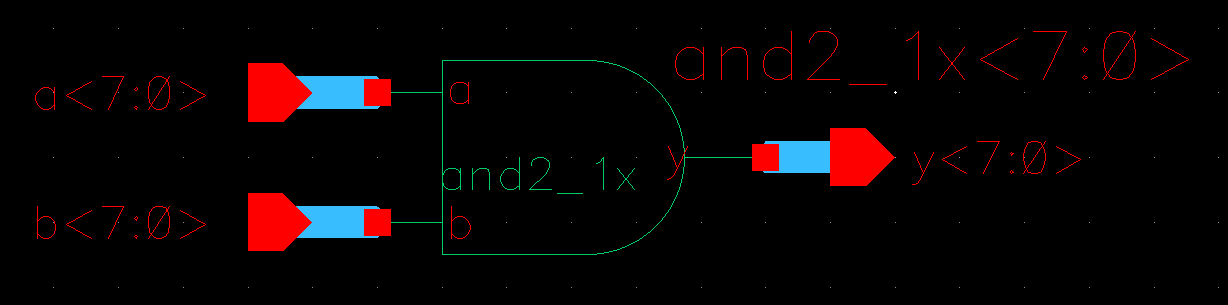
\includegraphics[width=0.5\textwidth]{and2_1x_8_schematic.png}}
		\caption{Schematic for AND Wordslice}
		\label{fig::and2_1x_8_schematic}
	\end{figure}
	
	\noindent Next, we create a symbol for our AND wordslice. For this step, we start with a copy of the \texttt{and2\_1x} symbol and make small incremental updates. Our wordslice symbol with these updates is shown in Figure \ref{fig::and2_1x_8_symbol}. Note that the port names and wire widths have been updated to reflect the vectorized inputs and outputs.
	
	\begin{figure}[H]
		\centerline{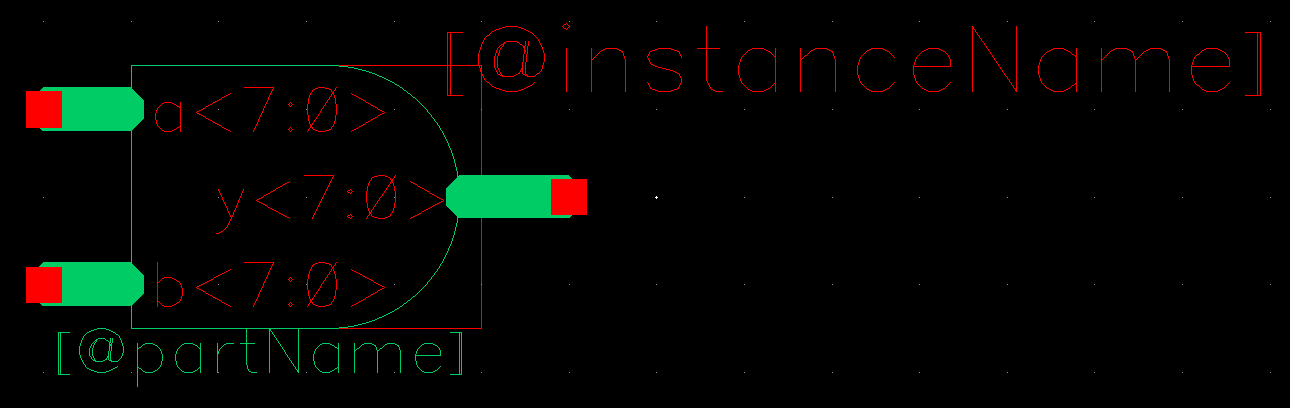
\includegraphics[width=0.5\textwidth]{and2_1x_8_symbol.png}}
		\caption{Symbol for AND Wordslice}
		\label{fig::and2_1x_8_symbol}
	\end{figure}
	
	\noindent Then, we create a layout for our wordslice. To create the layout, we start with a mosiac of AND gates. The resulting layout with different display levels is shown in Figures \ref{fig::and2_1x_8_layout_mosiac_overview} and \ref{fig::and2_1x_8_layout_detailed}.
	
	\begin{figure}[H]
		\centerline{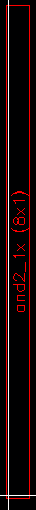
\includegraphics[height=0.8\textwidth, angle=270]{and2_1x_8_layout_mosiac_overview.png}}
		\caption{AND Gate Mosiac Layout Display Level = 0}
		\label{fig::and2_1x_8_layout_mosiac_overview}
	\end{figure}
	
	\begin{figure}[H]
		\centerline{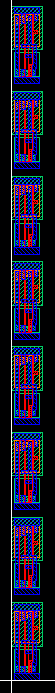
\includegraphics[height=0.8\textwidth, angle=270]{and2_1x_8_layout_detailed.png}}
		\caption{AND Gate Mosiac Layout Display Level = 1}
		\label{fig::and2_1x_8_layout_detailed}
	\end{figure}
	
	\noindent In the layouts, we placed input and output ports for each of the gates. However, in this configuration, virtuoso shorted each element within the vector of pins. These shorts are displayed on an individual AND gates in Figure \ref{fig::and2_1x_8_cell_with_shorts} and in the Annotation Browser in Figure \ref{fig::and2_1x_8_annotation_shorts}. 
	
	\begin{figure}[H]
		\centerline{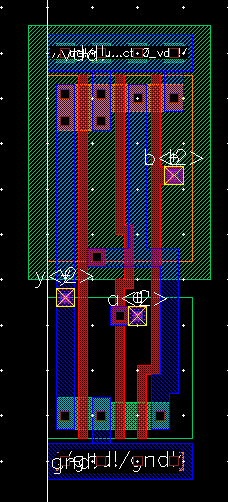
\includegraphics[width=0.2\textwidth]{and2_1x_8_cell_with_shorts.png}}
		\caption{Shorts Marked in the Schematic}
		\label{fig::and2_1x_8_cell_with_shorts}
	\end{figure}
	
	\begin{figure}[H]
		\centerline{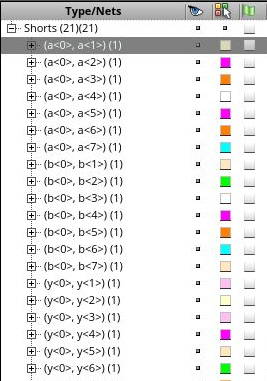
\includegraphics[width=0.35\textwidth]{and2_1x_8_annotation_shorts.png}}
		\caption{Shorts Called Out by the Annotation Browser}
		\label{fig::and2_1x_8_annotation_shorts}
	\end{figure}
	
	\noindent To work around this, I instantiated a single AND gate and then copied it 7 times with $33{\mu}m$ spacing. The resulting schematic at display level = 0 is shown in Figure \ref{fig::and2_1x_8_layout_overview}. Note that the AND gates are now displayed individually at this display level = 0, but the instantiated gates should be identical.
	
	\begin{figure}[H]
		\centerline{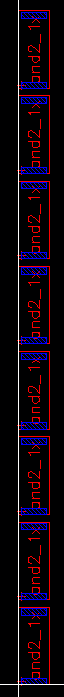
\includegraphics[height=0.8\textwidth, angle=270]{and2_1x_8_layout_overview.png}}
		\caption{AND Wordslice Created without Mosiac at Display Level = 0}
		\label{fig::and2_1x_8_layout_overview}
	\end{figure}
	
	\noindent We also highlight the port placement for a single AND gate, which is shown in Figure \ref{fig::and2_1x_8_single_gate_ports}.
	
	\begin{figure}[H]
		\centerline{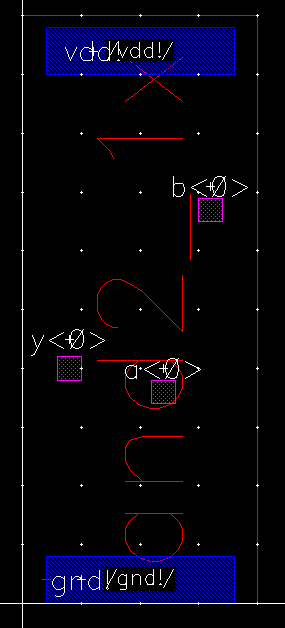
\includegraphics[width=0.25\textwidth]{and2_1x_8_single_gate_ports.png}}
		\caption{Port Placement for a Given AND Gate}
		\label{fig::and2_1x_8_single_gate_ports}
	\end{figure}
	
	\noindent Next, we wanted to verify our design with DRC and LVS. According to the installed Cadence documentation, this should be done with Verify \textgreater\ DRC and Verify \textgreater\ LVS in the layout window. However, the Verify drop-down menu did not include these options. As a result, I was unable to perform DVS and LVS at the rigor I wanted.
	
	\begin{figure}[H]
		\centerline{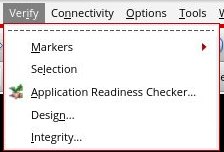
\includegraphics[width=0.4\textwidth]{verify_dropdown_menu.png}}
		\caption{Verify Drop-Down Menu in Layout Window}
		\label{fig::verify_dropdown_menu}
	\end{figure}
	
	\begin{figure}[H]
		\centerline{\fbox{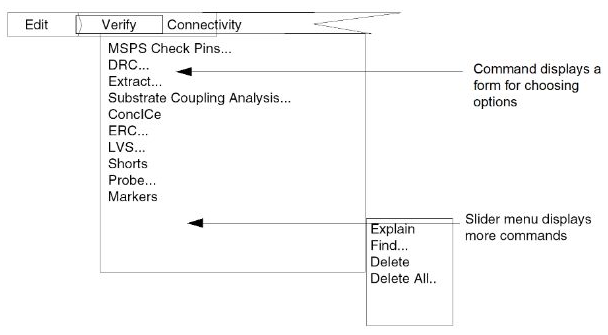
\includegraphics[height=0.4\textwidth]{verify_dropdown_menu_doc.png}}}
		\caption{Verify Drop-Down Menu per Documentation}
		\label{fig::verify_dropdown_menu_doc}
	\end{figure}
	
	\noindent Instead, I performed a reduced set of checks using Verify \textgreater\ Application Readiness Checker.... To get passing results I had to do two things. First, I had to associate each of the AND gates in the schematic with gates in my layout using Connectivity \textgreater\ Define Device Correspondence. Second, I had to create "Must Connect" groups for gnd! and vdd!, which I did with Pins \textgreater\ Pin Connectivity Setting.... My final application readiness checks are shown in Figure \ref{fig::and_application_readiness_check}.
	
	\begin{figure}[H]
		\centerline{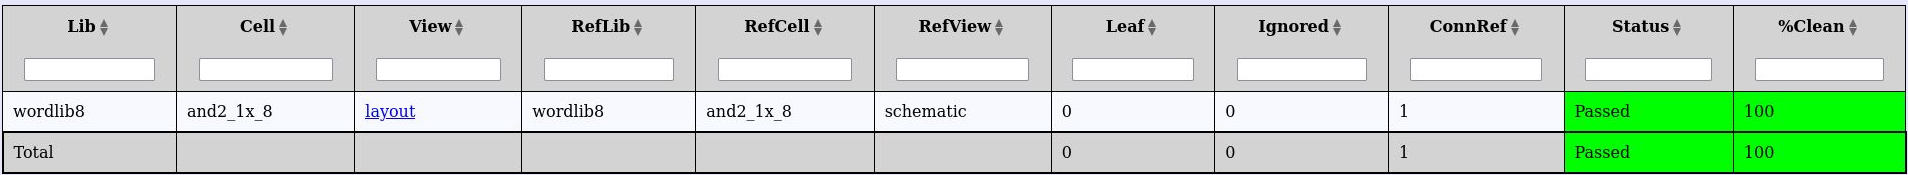
\includegraphics[width=0.9\textwidth]{and_application_readiness_check.png}}
		\caption{Application Readiness Check Results}
		\label{fig::and_application_readiness_check}
	\end{figure}
	
	\noindent I also was able to use Verify \textgreater\ Design to populate the DRC annotations in the annotation browser. These annotations are shown in Figure \ref{fig::and_drc} and confirm no DRC failures.
	
	\begin{figure}[H]
		\centerline{\fbox{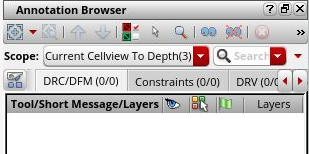
\includegraphics[width=0.5\textwidth]{and_drc.png}}}
		\caption{DRC Annotations Showing All Checks Passing}
		\label{fig::and_drc}
	\end{figure}
	
	\section{OR Wordslice}
	
	We repeat the process given in Section \ref{section::and_wordslice} to create an OR wordslice.  Our wordslice specifically contains 8 \texttt{or2\_1x} gates from the \texttt{muddlib11} library. The resulting schematic is shown in Figure \ref{fig::or2_1x_8_schematic}. Note the vectorized ports and component instances.
	
	\begin{figure}[H]
		\centerline{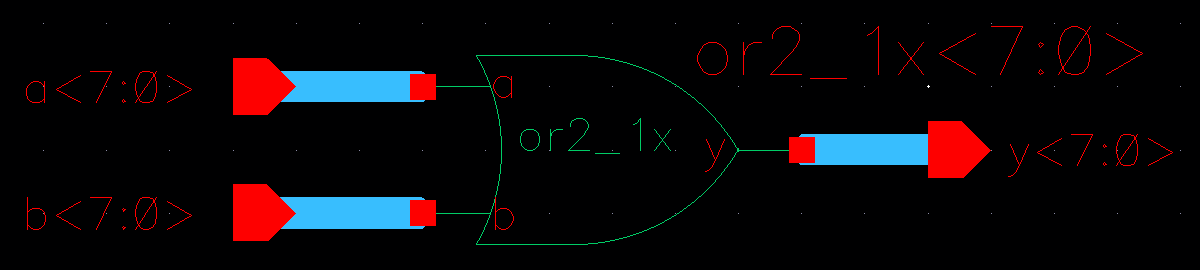
\includegraphics[width=0.5\textwidth]{or2_1x_8_schematic.png}}
		\caption{Schematic for OR Wordslice}
		\label{fig::or2_1x_8_schematic}
	\end{figure}
	
	\noindent Next, we create a symbol for our OR wordslice. For this step, we start with a copy of the \texttt{or2\_1x} symbol and make small incremental updates. Our wordslice symbol with these updates is shown in Figure \ref{fig::or2_1x_8_symbol}. Note that the port names and wire widths have been updated to reflect the vectorized inputs and outputs.
	
	\begin{figure}[H]
		\centerline{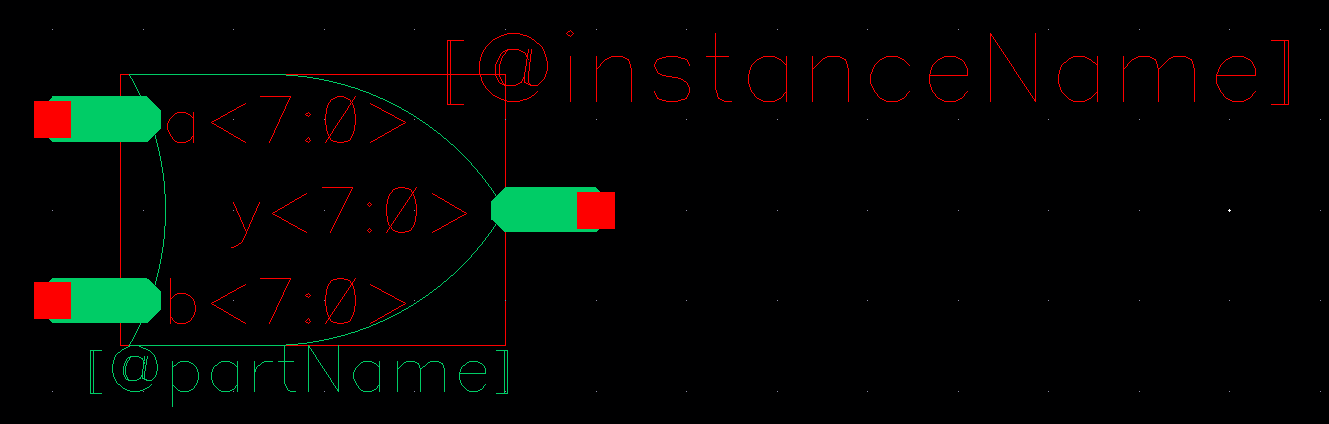
\includegraphics[width=0.5\textwidth]{or2_1x_8_symbol.png}}
		\caption{Symbol for OR Wordslice}
		\label{fig::or2_1x_8_symbol}
	\end{figure}
	
	\noindent Tehen, we create a layout for our wordslice. We leverage what we learned from the previous section and copy OR gates instead of using a mosiac. This helps us to prevent unintentional shorts. The layout with different display levels is shown in Figures \ref{fig::or2_1x_8_layout_overview} and \ref{fig::or2_1x_8_layout_detailed}.
	
	\begin{figure}[H]
		\centerline{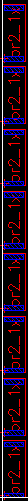
\includegraphics[height=0.8\textwidth, angle=270]{or2_1x_8_layout_overview.png}}
		\caption{OR Wordslice Layout Display Level = 0}
		\label{fig::or2_1x_8_layout_overview}
	\end{figure}
	
	\begin{figure}[H]
		\centerline{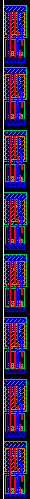
\includegraphics[height=0.8\textwidth, angle=270]{or2_1x_8_layout_detailed.png}}
		\caption{OR Wordslice Layout Display Level = 1}
		\label{fig::or2_1x_8_layout_detailed}
	\end{figure}
	
	\noindent We also highlight the port placement for a single OR gate, which is shown in Figure \ref{fig::or2_1x_8_single_gate_ports}.
	
	\begin{figure}[H]
		\centerline{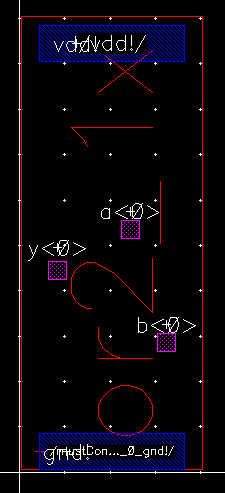
\includegraphics[width=0.25\textwidth]{or2_1x_8_single_gate_ports.png}}
		\caption{Port Placement for a Given OR Gate}
		\label{fig::or2_1x_8_single_gate_ports}
	\end{figure}
	
	\noindent Next, following the work from the previous section, we perform application readiness checks and check the annotations browser for DRC failures. To avoid errors in the application readiness checks, we map gates in the schematic to gates in the layout and create "Must Connect" groups for gnd! and vdd! The application readiness checks shown in Figure \ref{fig::or_application_readiness_check} and DRC checks shown in Figure \ref{fig::or_drc} show no errors.
	
	\begin{figure}[H]
		\centerline{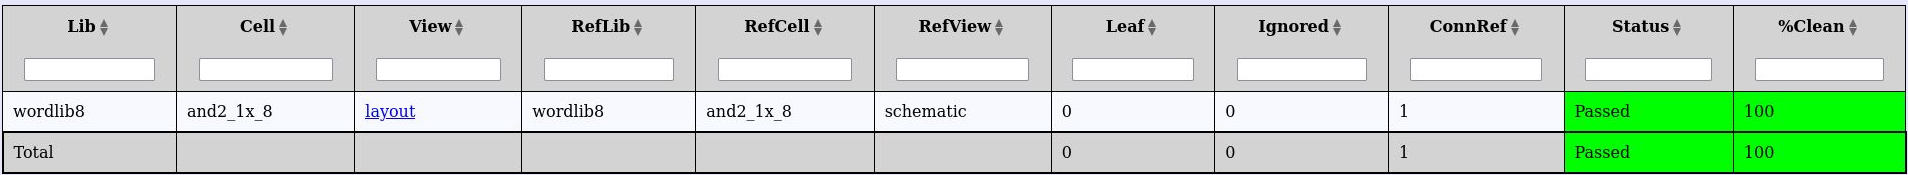
\includegraphics[width=0.9\textwidth]{and_application_readiness_check.png}}
		\caption{Application Readiness Check Results}
		\label{fig::or_application_readiness_check}
	\end{figure}
	
	\begin{figure}[H]
		\centerline{\fbox{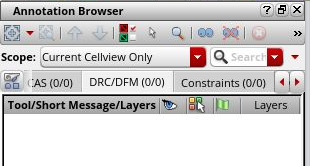
\includegraphics[width=0.5\textwidth]{or_drc.png}}}
		\caption{DRC Annotations Showing All Checks Passing}
		\label{fig::or_drc}
	\end{figure}
	
	\section{ALU}
	
	In this section, we complete the ALU schematic using the AND and OR wordslices we created in the previous sections. The resulting schematic is shown in Figure \ref{fig::alu_schematic}.
	
	\begin{figure}[H]
		\centerline{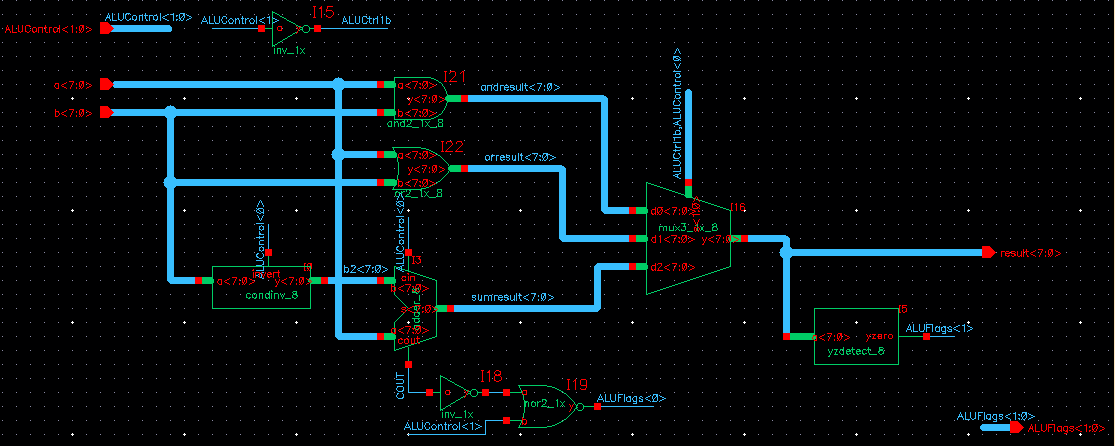
\includegraphics[width=0.9\textwidth]{alu_schematic.png}}
		\caption{ALU Schematic after Adding AND and OR Wordslices}
		\label{fig::alu_schematic}
	\end{figure}
	
	\noindent Then, we modify the ALU layout to include the AND and OR wordslices. The layout with different display levels is shown in Figures \ref{fig::alu_layout_overview} and \ref{fig::alu_layout_detailed}. The AND wordslice (top) and OR wordslice (bottom) are highlighted in both of the layouts. Before rotation, the AND gate is on the left and the OR gate is on the right.
	
	\begin{figure}[H]
		\centerline{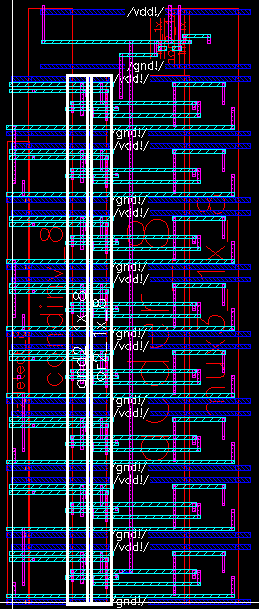
\includegraphics[height=0.8\textwidth, angle=270]{alu_layout_overview.png}}
		\caption{ALU Layout Display Level = 0}
		\label{fig::alu_layout_overview}
	\end{figure}
	
	\begin{figure}[H]
		\centerline{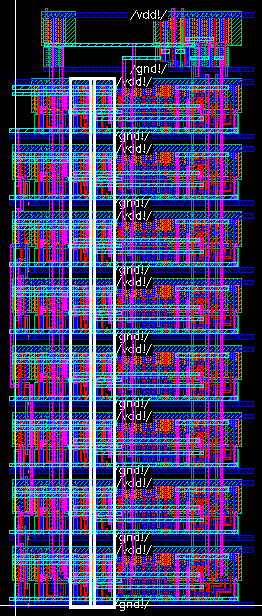
\includegraphics[height=0.8\textwidth, angle=270]{alu_layout_detailed.png}}
		\caption{ALU Layout Display Level = 1}
		\label{fig::alu_layout_detailed}
	\end{figure}
	
\end{document}